%------------------------------------
% 5) Função logarítmica f(x) = ln x
%------------------------------------

\begin{figure}[H]
  \centering
  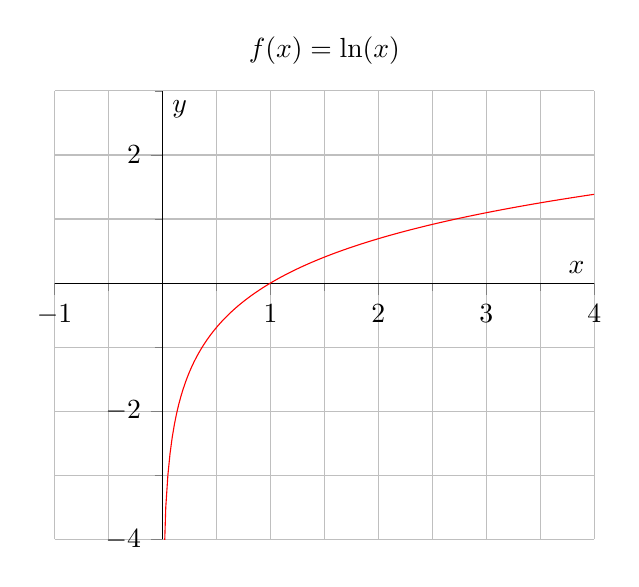
\begin{tikzpicture}
    \begin{axis}[
      xmin=-1, xmax=4,
      ymin=-4, ymax=3,
      axis x line=middle,
      axis y line=middle,
      axis line style={-},
      tick align=outside,
      grid=both,
      minor tick num=1,
      xlabel={$x$},
      ylabel={$y$},
      title={$f(x)=\ln(x)$}
    ]
      \addplot[red, domain=0.01:4, samples=200] {ln(x)};
    \end{axis}
  \end{tikzpicture}
  \caption{Função logarítmica natural $f(x)=\ln(x)$.}
\end{figure}